\documentclass{article}

\usepackage{ctex}
\usepackage{amsmath}
\usepackage{amssymb}
\usepackage{amsthm}
\usepackage{amsfonts}
\usepackage{graphicx}
\usepackage{float}

\usepackage[a4paper, left=1in, right=1in, top=1in, bottom=1in]{geometry}

\title{\textbf{数学与现代音乐}}
\author{曹陈都 3230104276}
\date{\today}

\begin{document}

\maketitle

\begin{abstract}
\label{abstract}
本文探究了现代音乐在分析与创作中蕴含的数学规律。通过集合论、抽象代数等非传统的数学音乐方法,我们得以更深入地理解音乐的结构和形式。通过特定的算法与生成模型,我们还可以将数学方法用于实际的音乐创作,实现数学与音乐的深刻交融。
\end{abstract}

\section{引言}
\label{sec:introduction}
数学自古以来就与音乐有着密切的联系。早在古希腊时期,毕达哥拉斯就发现了音高与弦长之间的比例关系:当琴弦弦长减半时,音高就会提高一个八度\cite{math_history_2017}。两根按特定比例调好的琴弦发出的声音将会是“协和”的,例如八度音程、五度音程等,这些比例关系可以用整数比来表示。对于毕达哥拉斯及其学派的古希腊人来说,数学与音乐存在着如此天然的和谐关系。

毕达哥拉斯在此基础上还提出了"五度相生律(Pythagorean Tuning)",这是最早而最为广泛应用的律制之一。其以一个基础音为起点,通过频率比为3:2的五度音程连续相生,从而推导出音阶中的其他音。但五度相生循环12次之后,得到的音高与起始音的八度音存在了一个较小的偏差,这个偏差被称为"毕式音差",在特定情况下影响了音乐的和谐性。

律制经过长时间的发展,最终演变成了“十二平均律(Equal Temperament)”这一较为完备的形式。最早发现十二平均律的是我国明代的学者朱载堉,而将其在音乐创作中发扬光大的是“音乐之父”巴赫。十二平均律将一个八度音程分为12个等分音程,使得每个音程的频率比为$\sqrt[12]{2}$,从而消除了毕式音差。这一律制的广泛应用使得音乐创作和演奏变得更加灵活和多样化\cite{math_art_2021}。

\section{音高集合论}
\label{sec:pitch_set_theory}
20世纪初期,在“调性危机”的时代背景下,以勋伯格(Arnold Schoenberg)为首的一批音乐家开始了“无调性”音乐的创作。“无调性”音乐并不同其字面意思给人的第一印象,它不是一种完全没有秩序的音乐,恰好相反,它有着非常严谨的规则。在勋伯格的音乐体系中,12个乐音可以以任何次序排列,不重复的几个音的特定组合方式称为“序列(series)”。在每一个序列中,音高之间的地位是完全平等的,而不是像传统的调性音乐一样,每个音符都跟某个“主音”有着特定的音乐关联,重要的是每个音符相对于之前音符的位置,这与爱因斯坦的相对论有着异曲同工之妙\cite{how_music_is_made_2021}。

以勋伯格这样的思想为核心诞生的音乐被称为"序列主义(Serialism)"。除了勋伯格及其弟子韦伯恩(Anton Webern)和贝尔格(Alban Berg)做出的巨大贡献之外,法国作曲家奥利维埃·梅西安(Olivier Messiaen)和其弟子皮埃尔·布列兹(Pierre Boulez)等人在序列主义的基础上继续发展出了新的音乐语言,他们不仅泛化了音高,同时还泛化了时值、力度、音色、奏法等要素,使得音乐创作的自由度进一步提高。以梅西安为主要代表的新流派被称为"整体序列主义(Integral Serialism)"。

\begin{figure}[h!]
    \centering
    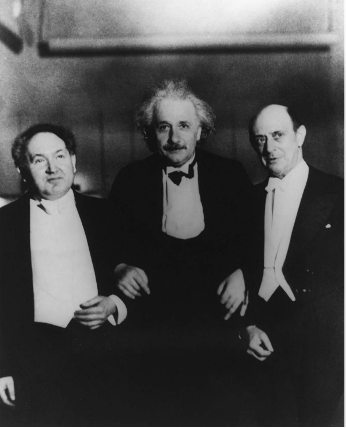
\includegraphics[width=0.8\textwidth]{image/im1.png}
    \caption{1934 年,爱因斯坦和勋伯格在纽约的卡内基音乐厅。}
    \label{fig:einstein_schoenberg}
\end{figure}

为了分析勋伯格及其后继者的音乐,音乐学家们发展出了“音高集合论(Pitch Set Theory)”。这最早由米尔顿·巴比特(Milton Babbitt)在二十世纪六十年代提出\cite{babbitt1960}\cite{babbitt1961}。音高集合论的核心思想是将音高视为一个集合,称为“音级集合(Pitch-Class Set)”,简称 PC Set\cite{forte_structure_2007}。

我们将十二平均律中的12个音高集合用整数 0 到 11 来表示。通常,C=0
\[
    C=0, C\sharp/D\flat=1, D=2, E\flat=3, E=4, F=5, F\sharp=6, G=7, A\flat=8, A=9, B\flat=10, B=11
\]

据此,一个C大三和弦(C,E,G)可以表示为集合 $\{0, 4, 7\}$。音级集合是无序集,因此 $\{0, 4, 7\}$ 和 $\{4, 7, 0\}$ 是同一个集合,它们都表示C大三和弦。并且在12音级数系统中,12与0是同一个音高,因此对于一个音级数我们将其加上12,其音高是保持不变的,所以$\{4, 7, 0\}$ 和 $\{4, 7, 12\}$相同。

从上面例子也可以看到,对于不同的音高集合,它们在某些情况下可能指向的是同一个和弦,因此我们需要在数学上探究一种形式去进行不同集合之间的比较,这便是音级集合的原型(Prime Form)。一个音级集合的原型,为了便于比较,其第一个数我们往往令其为0,但更重要的是,原型需要是一个\textbf{最佳标准序}。标准序指的是,先将一个PC Set中的元素按mod 12的顺序排列,然后列出以此顺序循环的所有可能的排列,取这些所有可能排列中第一个数与最后一个数差距最小的作为标准序。

\begin{align*}
    A_0 && [0, 2, 4, 8] && 8 \\
    A_1 && [2, 4, 8, 12] && 10 \\
    A_2 && [4, 8, 12, 14] && 10 \\
    A_3 && [8, 12, 14, 16] && 8
\end{align*}

对于此例子,我们可以看出$A_0$与$A_3$都是标准序,但$A_0$由于各相邻音级之间的距离较小,因此它是最佳标准序。且其第一个数字为0,因此我们将$A_0$作为原型。

对于每一个音级集合,我们存在两种运算,\textbf{移位}和\textbf{反行}。移位是指将集合中每一个数字加上一个整数 $n$ (最好mod12),反行是指将集合中每一个数字取模12后再取其补数。所有可以通过移位和反行互相得到的音级集合,我们视之为\textbf{等价}的\cite{schoenberg_introduction_2014}。

\begin{figure}[h!]
    \centering
    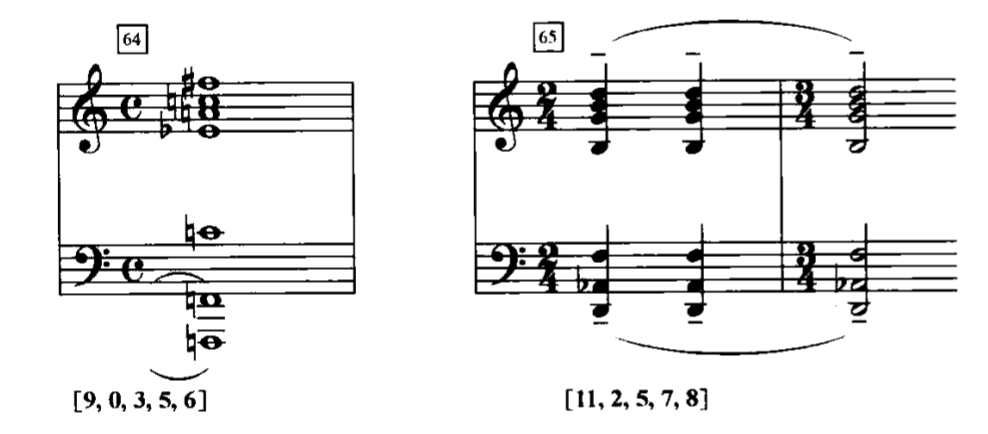
\includegraphics[width=0.8\textwidth]{image/im2.png}
    \caption{节选:贝尔格的《阿尔滕堡之歌》与斯特拉文斯基的《管乐交响乐》}
    \label{fig:berg_stravinsky}
\end{figure}

\begin{align*}
    \textbf{贝尔格:} \{9, 0, 3, 5, 6\} & \rightarrow \textbf{标准序} [3, 5, 6, 9, 0] & \rightarrow \textbf{移位} [0, 2, 3, 6, 9] &\xrightarrow{\text{移位/反行变换}} \textbf{原型} [0, 1, 3, 6, 9] \\
    \textbf{斯特拉文斯基:} \{11, 2, 5, 7, 8\} & \rightarrow \textbf{标准序} [5, 7, 8, 11, 2] & \rightarrow \textbf{移位} [0, 2, 3, 6, 9] &\xrightarrow{\text{移位/反行变换}} \textbf{原型} [0, 1, 3, 6, 9]
\end{align*}

我们可以看出,虽然贝尔格与斯特拉文斯基在音乐创作中使用了不同的音级集合,但它们的原型是相同的,这表明它们在音乐结构是等价的。由此我们可以看出,面对复杂的无调性音乐,音高集合论是分析其音乐内在原理的有力工具。

\section{抽象代数}
在音高集合论的基础上,抽象代数,特别是\textbf{群论}(Group Theory),为我们提供了严谨描述移位和反行变换的数学框架\cite{lewin1987gmit}。

对于移位运算,12音级的PC Set可以看成一个$Z_{12}$循环群。我们记移位二元运算为$T_n$,$n$为一个音级。从音级集合中任取一个音高,对其进行移位操作后,它必然还处在12音级的集合之中,因此满足封闭性。

0作为集合的单位元存在,显然满足
\[
    \forall x , T_0(x) = x
\]

对于逆元,我们有
\[
    \forall x , T_{12-x}(x) = 0
\]

或者
\[
    \forall x , T_{x}(12-x) = 0
\]

且结合律是显然满足的
\[
    \forall x, m, n , T_m(T_n(x)) = T_{m+n}(x)
\]

因此这个$Z_{12}$循环群可以被良好地定义

据上,可以将移位$T_n$看作一个元素,$T_0$至$T_{11}$共有12个元素。同理定义12个广义反行(倒影)$I_n$,$I_0$至$I_{11}$也共有12个元素。

\[
    \forall x , T_{n}(x) = x + n (\bmod 12)
\]

\[
    \forall x , I_{n}(x) = n - x (\bmod 12)
\]

对于这24个运算构成的集合,我们可以构造一个$D_{12}$二面体群,其二元运算可以记作$\circ$,可以理解为两个函数的复合运算。通过这个二面体群,移位与反行运算就被良好地统一在了一起,具有更佳精妙的数学结构。

\section{偶然性与新发展}
勋伯格及其后继者的序列主义音乐极其具有严谨性,但是音乐界也存在着不同的声音,20世纪60年代,约翰·凯奇(John Cage)提出了“偶然性音乐(Chance Music)”的概念,强调音乐创作中的随机性和偶然性。他的代表作《4分33秒》便是一个典型的例子,这个作品中没有任何一个音符,全程演奏者只是静坐在台上,聆听周围的环境声音。毫无疑问这种音乐形式是非常前卫的,对严格的音乐创作形式带来了巨大的冲击力。

但对数学的世界来说,纯粹无迹可寻的“偶然性”是荒谬的,通过概率论与随机过程的数学工具,我们可以对偶然性进行建模,甚至进行预测和操作,这便是雅尼斯·泽纳基斯(Yannis Xenakis)在音乐创作中所做的工作。他将随机性的数学艺术应用于音乐创作,创造出了一种崭新的音乐语言\cite{xenakis1992formalized}。

泽纳基斯将音乐分解为基本的\textbf{声粒子(Sound Particles)},每个声粒子有音高、时值、力度和音色四个特征,可以用以下数学表达式表达

\[
    G = (h, d, i, t)
\]

在作品《皮托普拉克塔》中,泽纳基斯希望在音乐中模拟出气体分子的无规则运动,他将46件弦乐器声粒子化,以音高h类比气体分子运动速率v,使其满足麦克斯韦-玻尔兹曼分布(MB Distribution)的概率分布函数,从而进行音乐创作,大致音高概率密度形式如下

\[
    P(h) = C h^2 e^{- \beta h^2}
\]

通过这种方式,泽纳基斯摆脱了传统音乐或序列主义音乐中的“线性”概念,通过每一个声粒子之间的复杂交织,实现了宏伟的“声云效果”。

\begin{figure}[h!]
    \centering
    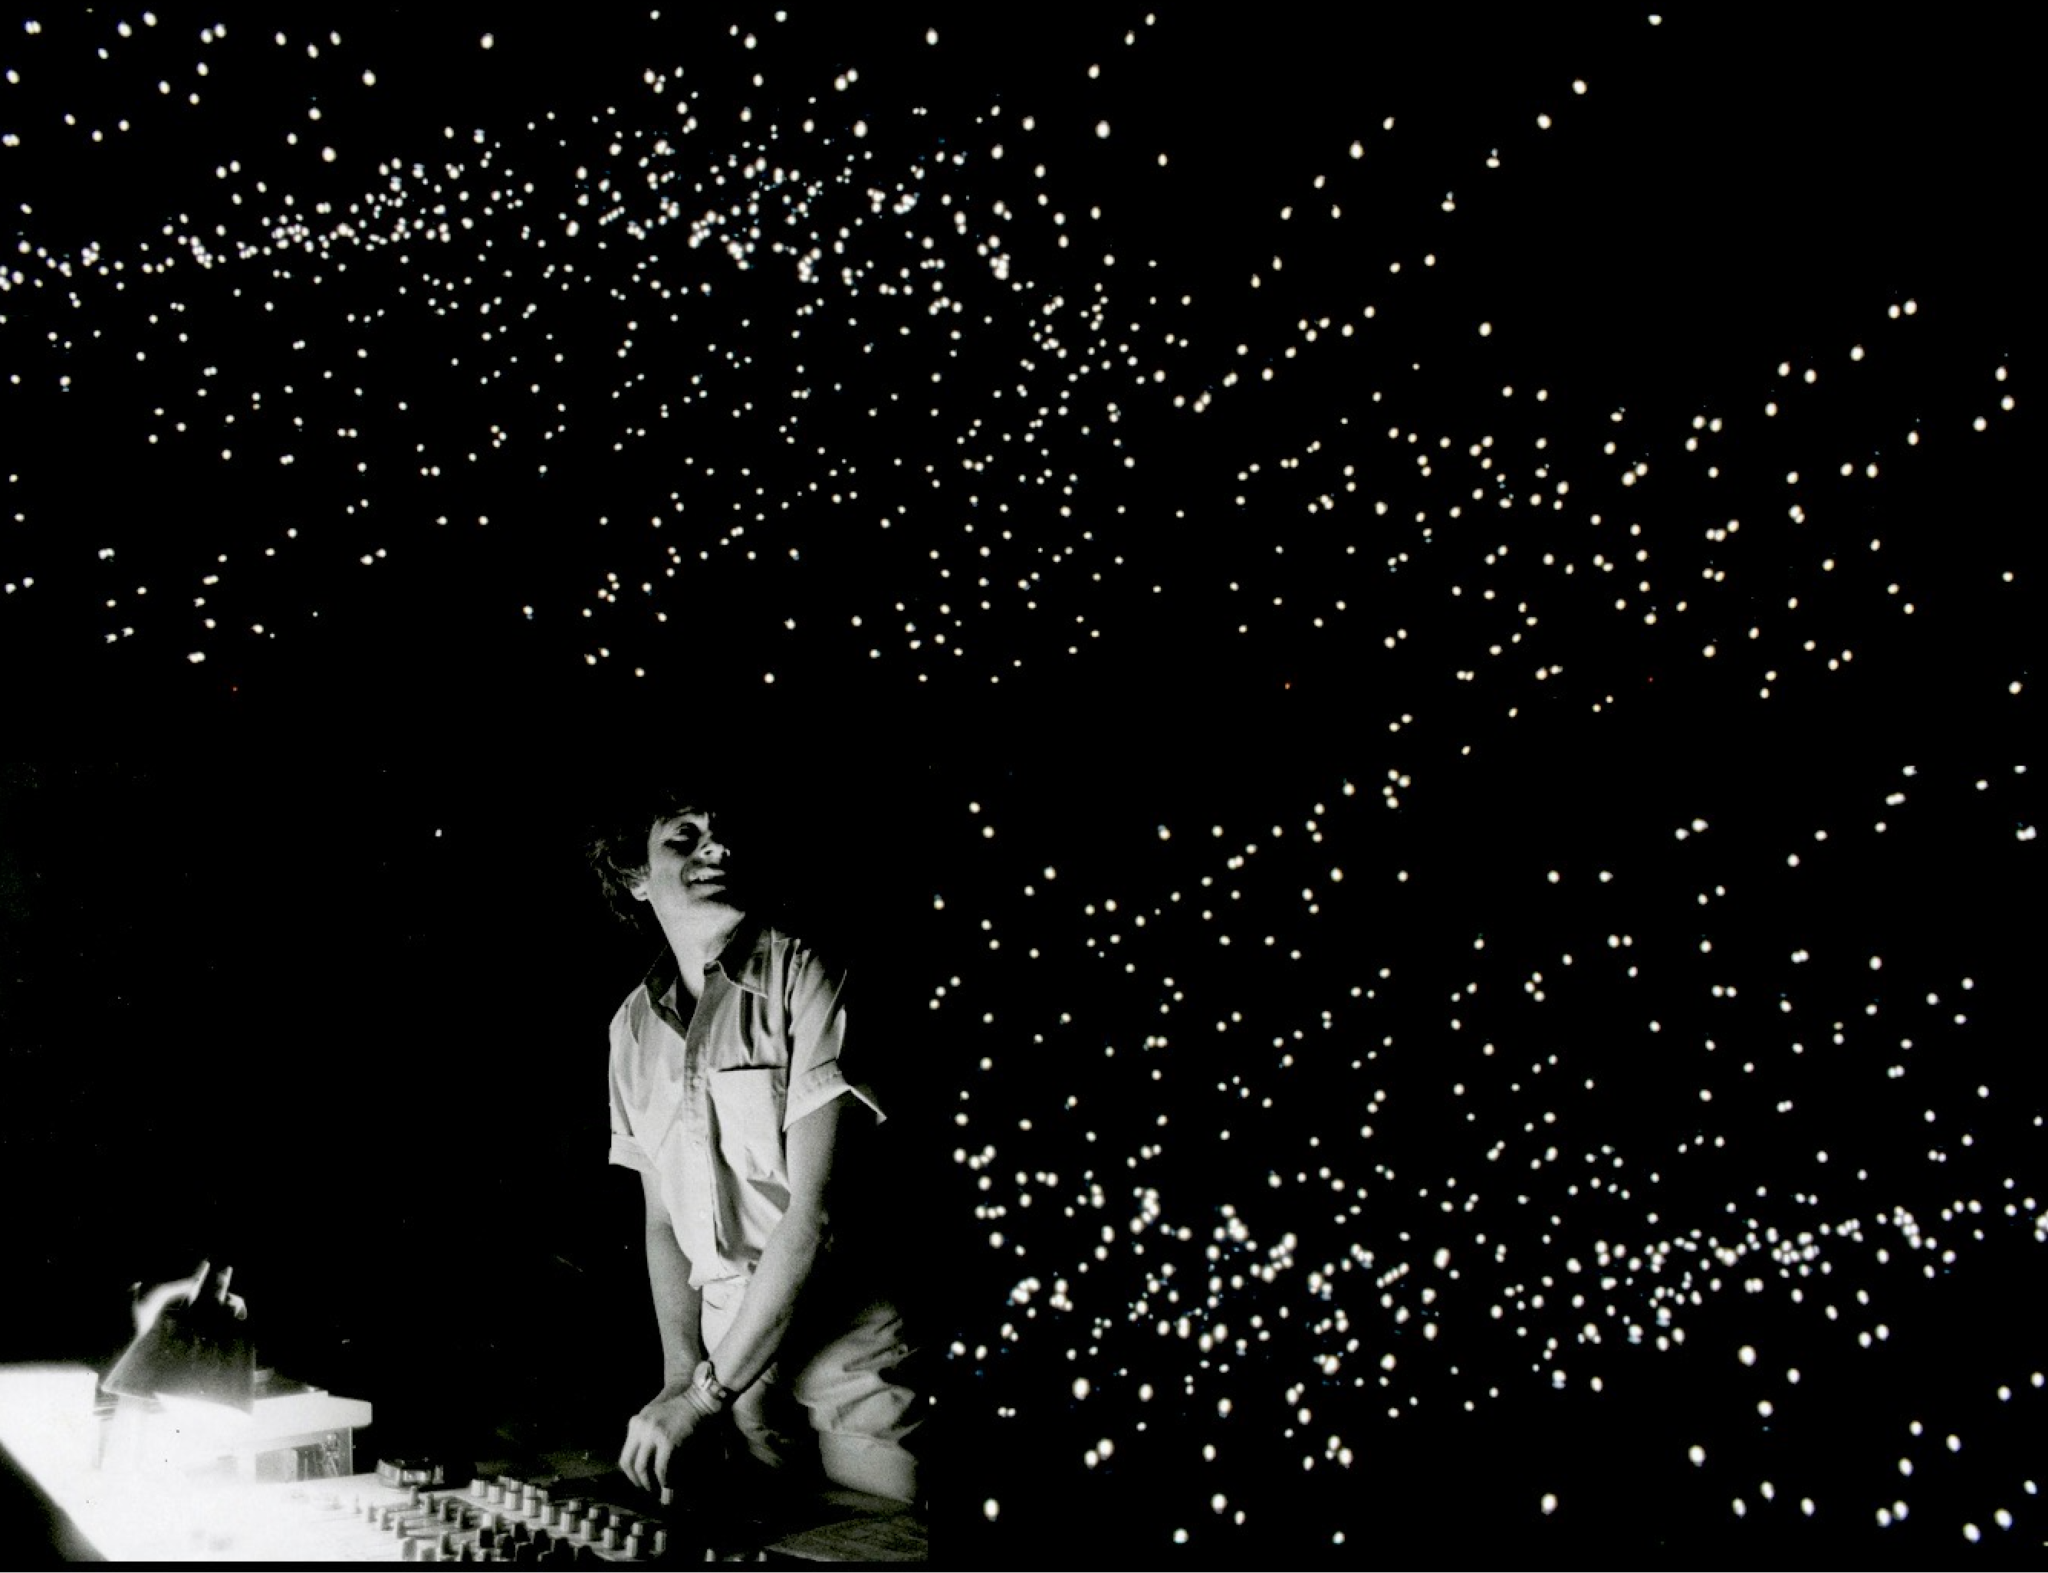
\includegraphics[width=0.8\textwidth]{image/im3.png}
    \caption{泽纳基斯与他的“声云”}
    \label{fig:xenakis_clouds}
\end{figure}

此外,马尔可夫链也被应用在泽纳基斯的音乐创作理念中,通过对每一个声粒子构建特定的转移概率矩阵,从而在一定程度上预测甚至控制“声云”的变换,并且使其能在时域上展开。

在约翰·凯奇的偶然性音乐中,他使用非常极端的随机过程方式进行音乐创造,例如《易经》占卜。但是泽纳基斯通过强大的数学工具,将这样的概率与随机过程量化了,并在统计意义下对其进行控制,这在音乐创作上是非常具有革新意义的。

同时,近年来人工智能的发展,也为音乐创作带来了更多的可能性。泽纳基斯的音乐思想深刻地影响了现在音乐大模型的构建,通过神经网络的训练和算法的优化,我们可以提高音乐的创作效率,开拓音乐的创作边界。

\section{结论与思考}
数学与音乐的关系是深刻而复杂的。经过上世纪至今不足百年的"风云变幻",数学音乐方法有着令人惊讶的突破,这首先是令人兴奋的。但是值得注意的一个问题就是,这样创作出的音乐"好听"吗?是否富有情感?这也是每一个音乐家都在试图去探寻的问题,因为音乐本质仍然是一种人文的情感的表达,而不是机械地进行声音变换。数学确实将音乐分析与创作技术化了,但不应该抹煞其中属于人的主观能动性。在未来,数学音乐方法也许会朝向这样一个方向发展:结合音乐心理学、认知科学甚至哲学,借助强大的数学工具,量化音乐与人的感官之间的相互作用,更加深入地探寻音乐的本质。我满怀希望地相信,数学、音乐以及人本能追求的美感与诗性是同构同源的,我们都是大自然的鬼斧神工。


\bibliography{reference.bib}
\bibliographystyle{plain}

\end{document}
